\documentclass[11pt,a4paper]{jsarticle}
\usepackage[dvipdfmx]{color}
\usepackage[dvipdfmx]{graphicx}
\usepackage{ascmac}
\usepackage[table,xcdraw]{xcolor}
\usepackage{float}
\usepackage{multicol}
\usepackage{listings,jlisting}
\renewcommand{\lstlistingname}{リスト}
\lstset{
	language=c,%
	basicstyle=\scriptsize,%
	numbersep=5pt,%
	breaklines=true,%
	breakindent=5pt,%
	frame=single,%
	tabsize=2,%
	numbers=left,%
	numberstyle=\tiny,%
	showstringspaces=false%
	}%
\setlength{\columnsep}{20pt}
\setlength{\columnwidth}{200cm}

\begin{document}
  % 表紙
  \begin{center}
    {\Large 平成30年度ソフトウェア設計\\ テトリスの作成}\par
    \vspace{15mm}
    {\today}\par
    \vspace{100mm}
    {\large 班名:10班}\par
    {\large 篠田拓樹(班長) 伊崎龍河(副班長) 秋元駿\\ 
    江尻姫花 尾畑賢太 本田歩 宮本雅也}
  \end{center}
  \thispagestyle{empty}
  \clearpage
  \addtocounter{page}{-1}
  % 目次
  \tableofcontents
  \clearpage
  % 本文
  \section{要求仕様}
    \begin{description}
  \item[目的] 娯楽を通して,脳の活性化をはかる
  \item[品質目標] 読みやすいコードを作成する
  \item[使用者の特性] 全年齢対象,キーボードが使えること,画面を視認できること
  \item[作るもの] テトリス
  \item[機能的要求] テトリスとして動作すること
  \item[動作環境・OS] Windows10
  \item[使用言語] C言語/C++
  \item[外部ライブラリ] DxLibrary(GUI表示用)
  \item[インターフェース] 標準キーボード,ディスプレイ
  \item[ネットワーク] なし
\end{description}

  \section{ルール}
    7種類のブロックからランダムに1つずつ落ちてくる.
落ちてくるブロックを操作(回転・左右下移動)する.
操作中のブロックが積み上げられたブロックに触れると
固定され,次のブロックが落ちてくる.
ブロックが固定されたときに1行揃ったらその行は,消える.
消えた行より上の行は,1行詰められる.
縦20行×横10列のフィールド上で行われる.
ブロックは,上から落ちてくる.落ちてくるスピードは,$1[block/s]$程度.
シンプルなテトリスを実装するため,回転によるはめ込み(T-Spin)や
対戦機能等は実装しないこととする.
ブロックの形は,4つの正方形を組み合わせたものである.
スコアアップについては,1行消すごとに1行:1倍,2行:1.25倍,3行:1.5倍,4行:1.75倍のように0.25倍ずつ増えることとする.

  \clearpage
  \section{計画表}
    以下に作成した計画表を示す.
上の表は計画段階での表であり,下の表は実際に行った作業の日程である.
表中の黒い部分が日程での作業である.

\begin{figure}[htb]
  \begin{center}
    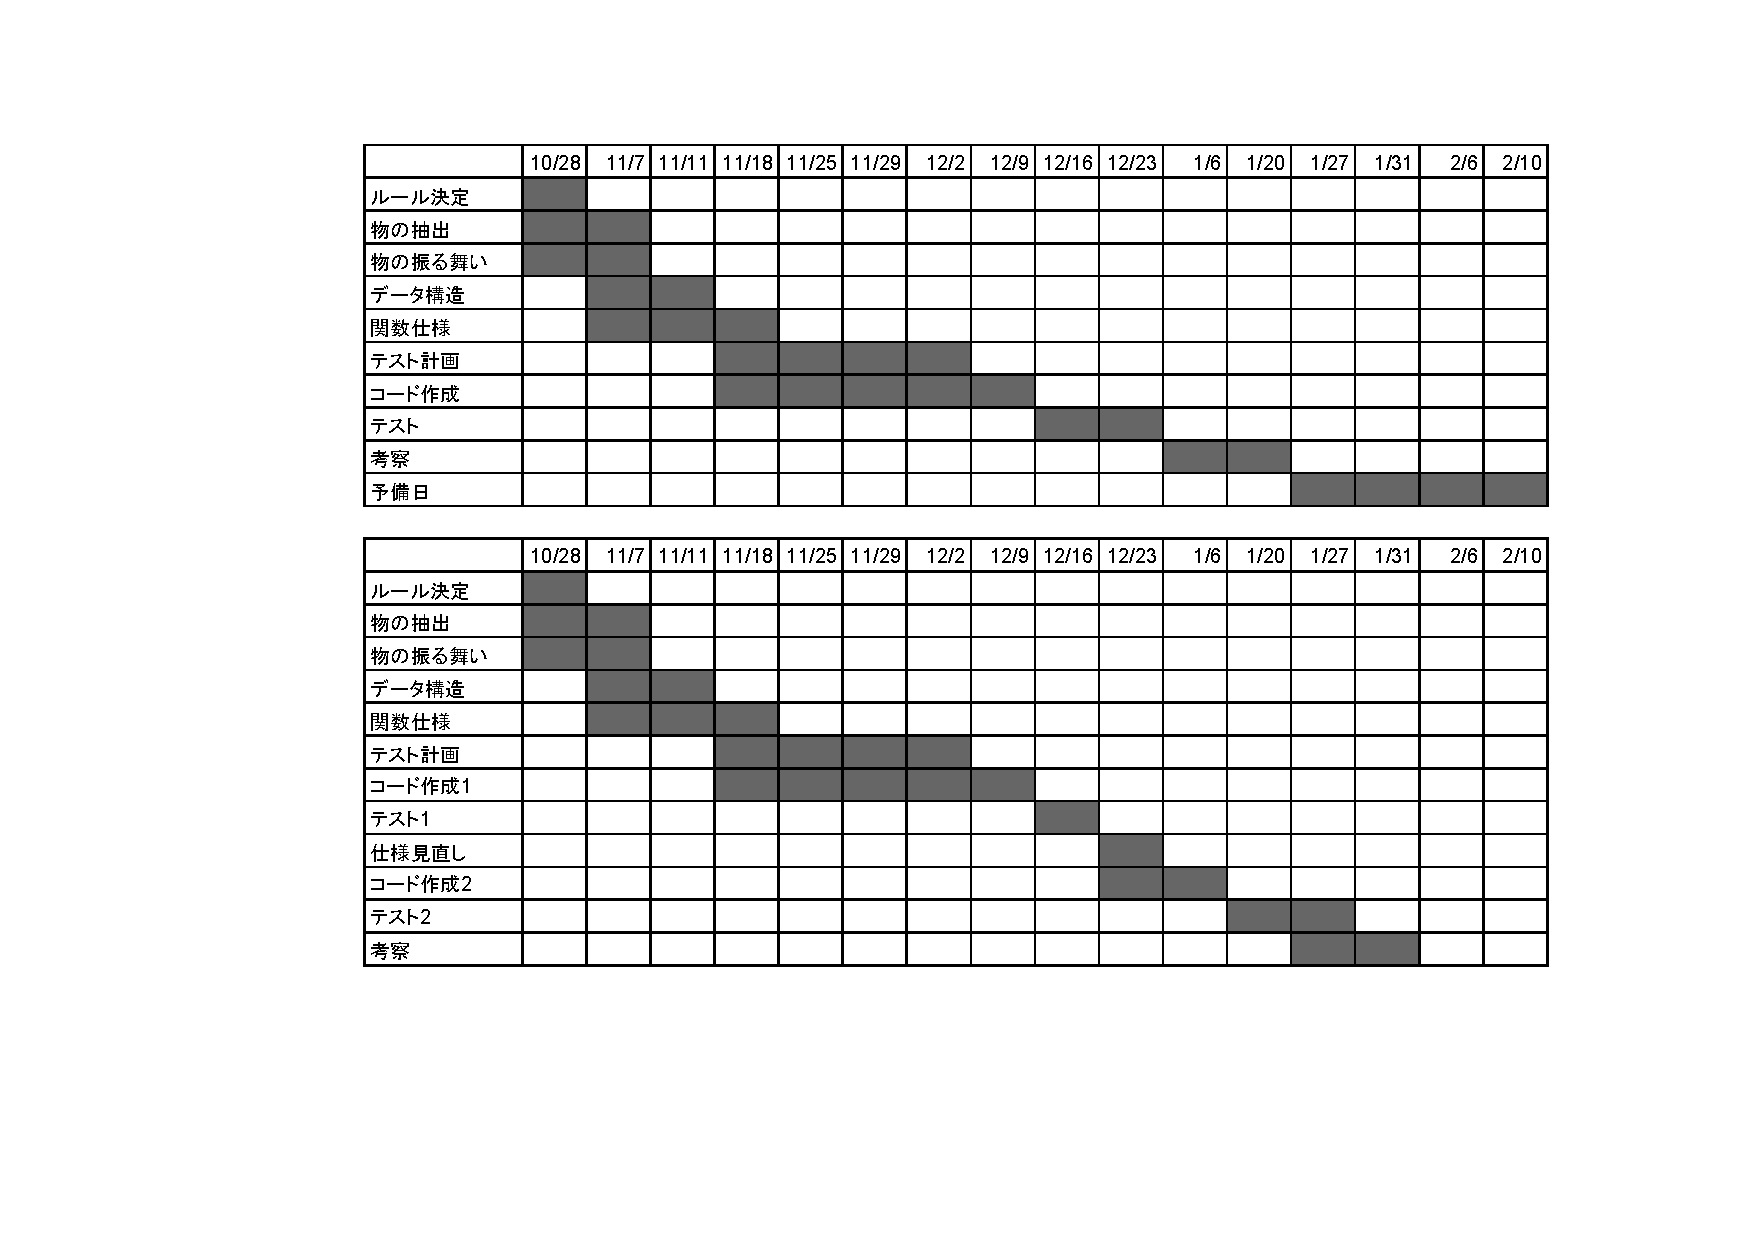
\includegraphics[scale=0.7,bb=150 106 765 544]{./img/plan_image.pdf}
  \end{center}
\end{figure}

  \section{役割分担}
    \begin{itemize}
  \item 物の抽出・振る舞い抽出:秋元・尾畑
  \item データ構造・関数仕様:秋元・尾畑
  \item テスト計画:本田
  \item コード作成:篠田
  \item テスト:宮本・伊崎
  \item 考察・まとめ:江尻・伊崎
  \item 資料作成:篠田
\end{itemize}

  \clearpage
  \section{テスト計画}
    \begin{table}[htb]
\begin{tabular}{|l|l|l|}
\hline
テスト内容                             & 1回目 & 2回目 \\ \hline
落ちてくるブロックがランダムであるか                & 正常  & 正常  \\ \hline
ブロックが7種類全て出現するか                   & 正常  & 正常  \\ \hline
ブロックがフィールドを出ないか                   & 正常  & 正常  \\ \hline
ブロックの操作(下左右移動ができるか)               & 正常  & 正常  \\ \hline
操作中のブロックが固定されるか                   & 正常  & 正常  \\ \hline
ブロック固定後に次のブロックが落ちてくるか             & 正常  & 正常  \\ \hline
ブロックの落ちてくる速度が1{[}block/sec{]}であるか & 正常  & 正常  \\ \hline
回転によるはめ込み等の複雑な処理が実装されていないか        & 正常  & 正常  \\ \hline
ブロックが1行揃ったら消えるか                   & 正常  & 正常  \\ \hline
ブロックが消えたら1行詰められているか               & 正常  & 正常  \\ \hline
ポイントアップがルール通りに行われているか             & 異常  & 正常  \\ \hline
\end{tabular}
\end{table}

  \clearpage
  \section{物の抽出とふるまい}
    \subsection{物の抽出}
  \begin{itemize}
    \item テトリミノ
    \item フィールド
    \item スコア
  \end{itemize}
\subsection{物の振る舞い}
  \begin{itemize}
    \item テトリミノ:回転する,時間経過で落下,横に動く,生成する,表示する
    \item フィールド:列を消す,列を詰める,テトリミノを固定する  
    \item スコア:加算する,表示する
  \end{itemize}

  \section{データ構造}
    \begin{itemize}
  \item ブロック\\ \mbox{}
        struct t\_mino\{\\
          int mino[MINO\_SIZE][MINO\_SIZE]; // MINOSIZE=4 ミノの形状を表す\\
          int x,y; // ミノの座標(左上のマスを規準)\\
        \}
  \item フィールド\\ \mbox{}
        int field[FIELD\_Y][FIELD\_X]; // FIELD\_X=10,FIELD\_Y=20
  \item スコア\\ \mbox{}
        int score;
\end{itemize}

  \clearpage
  \section{関数仕様}
    \begin{table}[htb]
\begin{tabular}{|l|l|}
\hline
関数名 & void init\_field(); \\ \hline
引数  & なし                  \\ \hline
戻り値 & なし                  \\ \hline
内容  & フィールドをすべて0で初期化      \\ \hline
\end{tabular}
\end{table}

\begin{table}[htb]
\begin{tabular}{|l|l|}
\hline
関数名 & bool is\_field\_over(t\_mino mino);                                           \\ \hline
引数  & mino : テトリミノの情報                                                               \\ \hline
戻り値 & \begin{tabular}[c]{@{}l@{}}true : フィールド内である\\ false :  フィールド外である\end{tabular} \\ \hline
内容  & テトリミノがフィールド内であるかを判定                                                           \\ \hline
\end{tabular}
\end{table}

\begin{table}[htb]
\begin{tabular}{|l|l|}
\hline
関数名 & bool is\_field\_over\_y(t\_mino mino);                                        \\ \hline
引数  & mino : テトリミノの情報                                                               \\ \hline
戻り値 & \begin{tabular}[c]{@{}l@{}}true : フィールド内である\\ false :  フィールド外である\end{tabular} \\ \hline
内容  & テトリミノがy軸でフィールド内であるかを判定                                                        \\ \hline
\end{tabular}
\end{table}

\begin{table}[htb]
\begin{tabular}{|l|l|}
\hline
関数名 & bool is\_field\_over\_x(t\_mino mino);                                        \\ \hline
引数  & mino : テトリミノの情報                                                               \\ \hline
戻り値 & \begin{tabular}[c]{@{}l@{}}true : フィールド内である\\ false :  フィールド外である\end{tabular} \\ \hline
内容  & テトリミノがx軸でフィールド内であるかを判定                                                        \\ \hline
\end{tabular}
\end{table}

\begin{table}[htb]
\begin{tabular}{|l|l|}
\hline
関数名 & bool is\_side\_hit (t\_mino mino);                                                            \\ \hline
引数  & mino : テトリミノの情報                                                                               \\ \hline
戻り値 & \begin{tabular}[c]{@{}l@{}}true : テトリミノがブロックとかぶっている\\ false :  テトリミノがブロックとかぶっている\end{tabular} \\ \hline
内容  & テトリミノがx軸でブロックと被っているか判定                                                                        \\ \hline
\end{tabular}
\end{table}

\begin{table}[htb]
\begin{tabular}{|l|l|}
\hline
関数名 & bool is\_down\_hit (t\_mino mino);                                                            \\ \hline
引数  & mino : テトリミノの情報                                                                               \\ \hline
戻り値 & \begin{tabular}[c]{@{}l@{}}true : テトリミノがブロックとかぶっている\\ false :  テトリミノがブロックとかぶっている\end{tabular} \\ \hline
内容  & テトリミノがy軸でブロックと被っているか判定                                                                        \\ \hline
\end{tabular}
\end{table}

\begin{table}[htb]
\begin{tabular}{|l|l|}
\hline
関数名 & void row\_check();  \\ \hline
引数  & なし                  \\ \hline
戻り値 & なし                  \\ \hline
内容  & すべての列に対して揃っているか確認する \\ \hline
\end{tabular}
\end{table}

\begin{table}[htb]
\begin{tabular}{|l|l|}
\hline
関数名 & void pack\_block(int row); \\ \hline
引数  & row : 列の番号                 \\ \hline
戻り値 & なし                         \\ \hline
内容  & 指定された列より上の列を1段詰める          \\ \hline
\end{tabular}
\end{table}

\begin{table}[htb]
\begin{tabular}{|l|l|}
\hline
関数名 & void row\_clear(int row); \\ \hline
引数  & row : 列の番号                \\ \hline
戻り値 & なし                        \\ \hline
内容  & 指定された列を消去する               \\ \hline
\end{tabular}
\end{table}

\begin{table}[htb]
\begin{tabular}{|l|l|}
\hline
関数名 & void stack\_block(t\_mino mino); \\ \hline
引数  & mino : テトリミノの情報                  \\ \hline
戻り値 & なし                               \\ \hline
内容  & ミノをフィールドに固定する                    \\ \hline
\end{tabular}
\end{table}

\begin{table}[htb]
\begin{tabular}{|l|l|}
\hline
関数名 & void disp\_field(); \\ \hline
引数  & なし                  \\ \hline
戻り値 & なし                  \\ \hline
内容  & フィールドを表示する          \\ \hline
\end{tabular}
\end{table}

\begin{table}[htb]
\begin{tabular}{|l|l|}
\hline
関数名 & void disp(t\_mino mino) \\ \hline
引数  & mino : テトリミノの情報         \\ \hline
戻り値 & なし                      \\ \hline
内容  & ゲーム画面の表示                \\ \hline
\end{tabular}
\end{table}

\begin{table}[htb]
\begin{tabular}{|l|l|}
\hline
関数名 & void disp\_game\_over() \\ \hline
引数  & なし                      \\ \hline
戻り値 & なし                      \\ \hline
内容  & ゲームオーバー画面の表示            \\ \hline
\end{tabular}
\end{table}

\begin{table}[htb]
\begin{tabular}{|l|l|}
\hline
関数名 & void initialize(t\_mino *mino) \\ \hline
引数  & *mino : ミノの情報                  \\ \hline
戻り値 & なし                             \\ \hline
内容  & ゲームの初期化                        \\ \hline
\end{tabular}
\end{table}

\begin{table}[htb]
\begin{tabular}{|l|l|}
\hline
関数名 & void move\_block(t\_mino *mino, char key[256])                           \\ \hline
引数  & \begin{tabular}[c]{@{}l@{}}*mino : ミノの情報\\ key[256] : キーの情報\end{tabular} \\ \hline
戻り値 & なし                                                                           \\ \hline
内容  & テトリミノ動かす                                                                     \\ \hline
\end{tabular}
\end{table}

\begin{table}[htb]
\begin{tabular}{|l|l|}
\hline
関数名 & void rotate\_block(t\_mino *mino) \\ \hline
引数  & *mino : ミノの情報                     \\ \hline
戻り値 & なし                                \\ \hline
内容  & テトリミノを回転する                        \\ \hline
\end{tabular}
\end{table}

\begin{table}[htb]
\begin{tabular}{|l|l|}
\hline
関数名 & void make\_t\_mino(t\_mino *mino) \\ \hline
引数  & *mino : ミノの情報                     \\ \hline
戻り値 & なし                                \\ \hline
内容  & テトリミノを作成する                        \\ \hline
\end{tabular}
\end{table}

\begin{table}[htb]
\begin{tabular}{|l|l|}
\hline
関数名 & void move\_right(t\_mino *mino) \\ \hline
引数  & *mino : ミノの情報                   \\ \hline
戻り値 & なし                              \\ \hline
内容  & テトリミノを右に動かす                     \\ \hline
\end{tabular}
\end{table}

\begin{table}[htb]
\begin{tabular}{|l|l|}
\hline
関数名 & void move\_left(t\_mino *mino) \\ \hline
引数  & *mino : ミノの情報                  \\ \hline
戻り値 & なし                             \\ \hline
内容  & テトリミノを左に動かす                    \\ \hline
\end{tabular}
\end{table}

\begin{table}[htb]
\begin{tabular}{|l|l|}
\hline
関数名 & void move\_down(t\_mino *mino) \\ \hline
引数  & *mino : ミノの情報                  \\ \hline
戻り値 & なし                             \\ \hline
内容  & テトリミノを下に動かす                    \\ \hline
\end{tabular}
\end{table}

\begin{table}[htb]
\begin{tabular}{|l|l|}
\hline
関数名 & void disp\_t\_mino(t\_mino *mino) \\ \hline
引数  & *mino : ミノの情報                     \\ \hline
戻り値 & なし                                \\ \hline
内容  & テトリミノを表示する                        \\ \hline
\end{tabular}
\end{table}

\begin{table}[htb]
\begin{tabular}{|l|l|}
\hline
関数名 & void init\_score() \\ \hline
引数  & なし                 \\ \hline
戻り値 & なし                 \\ \hline
内容  & スコアの初期化            \\ \hline
\end{tabular}
\end{table}

\begin{table}[htb]
\begin{tabular}{|l|l|}
\hline
関数名 & void add\_score(int lines) \\ \hline
引数  & lines : 消した列の数             \\ \hline
戻り値 & なし                         \\ \hline
内容  & 消えた列数に応じたスコアの加算            \\ \hline
\end{tabular}
\end{table}

\begin{table}[htb]
\begin{tabular}{|l|l|}
\hline
関数名 & void disp\_score() \\ \hline
引数  & なし                 \\ \hline
戻り値 & なし                 \\ \hline
内容  & スコアの表示             \\ \hline
\end{tabular}
\end{table}

  \clearpage
  \section{状態遷移}
    状態遷移表を表\ref{state}に示す.
状態遷移表を作成することでシステムにおいてやってはならないこと
を可視化することが出来た.また,今回作成することが出来なかったが
状態遷移図を作成することによってシステムの状態の流れを可視化すること
が出来,より具体的に画面遷移等の状態の変化を見ることが出来るようになる.

\begin{landscape}
\begin{table}[htb]
\centering
\caption{状態遷移表}
\label{state}
\footnotesize
\begin{tabular}{|l|l|l|l|l|l|l|l|l|l|}
\hline
状態番号 & 状態名          & 上下左右ボタン & \begin{tabular}[c]{@{}l@{}}テトリミノが\\ ブロックに触れた\end{tabular} & \begin{tabular}[c]{@{}l@{}}テトリミノが\\ 下の壁に触れた\end{tabular} & \begin{tabular}[c]{@{}l@{}}テトリミノが\\ 下左右の壁を超えた\end{tabular} & \begin{tabular}[c]{@{}l@{}}テトリミノが\\ ブロックに被った\end{tabular} & 行が揃っていた & 1秒経過 & なし                \\ \hline
S0   & テトリミノ操作可能    & S12     & S2                                                        & S2                                                       &                                                            &                                                           &         & S10  & S0                \\ \hline
S1   & テトリミノの生成     &         & S13                                                       &                                                          &                                                            &                                                           &         &      & S0                \\ \hline
S2   & テトリミノを固定     &         &                                                           &                                                          &                                                            &                                                           &         &      & S3                \\ \hline
S3   & 行が何列揃っているか確認 &         &                                                           &                                                          &                                                            &                                                           & S4      &      &                   \\ \hline
S4   & 行の削除         &         &                                                           &                                                          &                                                            &                                                           &         &      & S5                \\ \hline
S5   & 行を詰める        &         &                                                           &                                                          &                                                            &                                                           &         &      & S6                \\ \hline
S6   & スコアの倍率計算     &         &                                                           &                                                          &                                                            &                                                           &         &      & S7                \\ \hline
S7   & スコアの加算       &         &                                                           &                                                          &                                                            &                                                           &         &      & S1                \\ \hline
S8   & テトリミノを右に移動   &         &                                                           &                                                          &                                                            &                                                           &         &      & S0                \\ \hline
S9   & テトリミノを左に移動   &         &                                                           &                                                          &                                                            &                                                           &         &      & S0                \\ \hline
S10  & テトリミノを下に移動   &         &                                                           &                                                          &                                                            &                                                           &         &      & S0                \\ \hline
S11  & テトリミノを回転     &         &                                                           &                                                          &                                                            &                                                           &         &      & S0                \\ \hline
S12  & 範囲外判定        &         &                                                           &                                                          & S0                                                         & S0                                                        &         &      & \{S8,S9,S10,S11\} \\ \hline
S13  & ゲームオーバー(終了)  &         &                                                           &                                                          &                                                            &                                                           &         &      & S13               \\ \hline
\end{tabular}
\end{table}
\end{landscape}

  \clearpage
  \section{操作方法}
    \subsection{ゲーム開始操作}
実行ファイル(main.exe)をダウンロードする.
実行ファイルを実行する.ゲームが開始されたらゲーム内操作に
従って操作を行う.
\subsection{ゲーム終了操作}
GameOver画面が表示されたらウィンドウの×ボタンを押してウィンドウを閉じる.
\subsection{ゲーム内操作方法}
操作方法を以下に示す.
\begin{itemize}
  \item[右矢印] テトリミノを右に移動する
  \item[左矢印] テトリミノを左に移動する
  \item[上矢印] テトリミノを時計回りに回転する
  \item[下矢印] テトリミノを下に移動する
\end{itemize}

  \clearpage
  \section{実行画面}
    \subsection{ゲーム画面}
初期画面を図\ref{gamescreen}に示す.
ゲームを開始すると同時にテトリミノが落下を始める.
\subsection{テトリミノの落下}
テトリミノの落下を図\ref{fool}に示す.
テトリミノは,毎秒1ブロックの速さで落下する.
\subsection{テトリミノの固定}
テトリミノの固定を図\ref{stick}に示す.
テトリミノは,他のブロックや下の範囲に触れると固定される.
\subsection{テトリミノの新規作成}
テトリミノの新規作成を図\ref{new}に示す.
テトリミノが固定されると新しく操作可能なブロックが作成される.
\subsection{1行消去のスコア加算}
1行消去したときのスコア加算を図\ref{one1},\ref{one2}に示す.
1行消去されるとスコアが100加算される.
\subsection{2行消去のスコア加算}
2行消去したときのスコア加算を図\ref{two1},\ref{two2}に示す.
2行消去されるとスコアが100加算される.
\subsection{3行消去のスコア加算}
3行消去したときのスコア加算を図\ref{three1},\ref{three2}に示す.
3行消去されるとスコアが100加算される.
\subsection{4行消去のスコア加算}
4行消去したときのスコア加算を図\ref{tetoris},\ref{tetoris2}に示す.
4行消去されるとスコアが100加算される.
\subsection{ゲームオーバー画面}
ゲームオーバー画面を図\ref{gameover}に示す.
ブロックが新しく出たときに操作不可能だった場合固定される.

\begin{figure}[htb]
  \begin{center}
    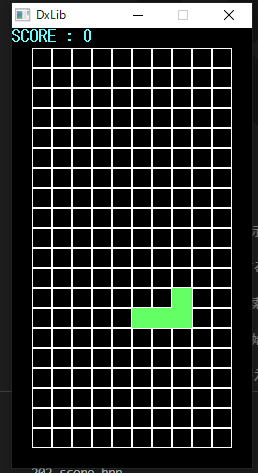
\includegraphics[scale=0.5]{./soft_img/gamescreen.png}
    \caption{ゲーム画面}
    \label{gamescreen}
  \end{center}
\end{figure}
\begin{figure}[htb]
  \begin{center}
    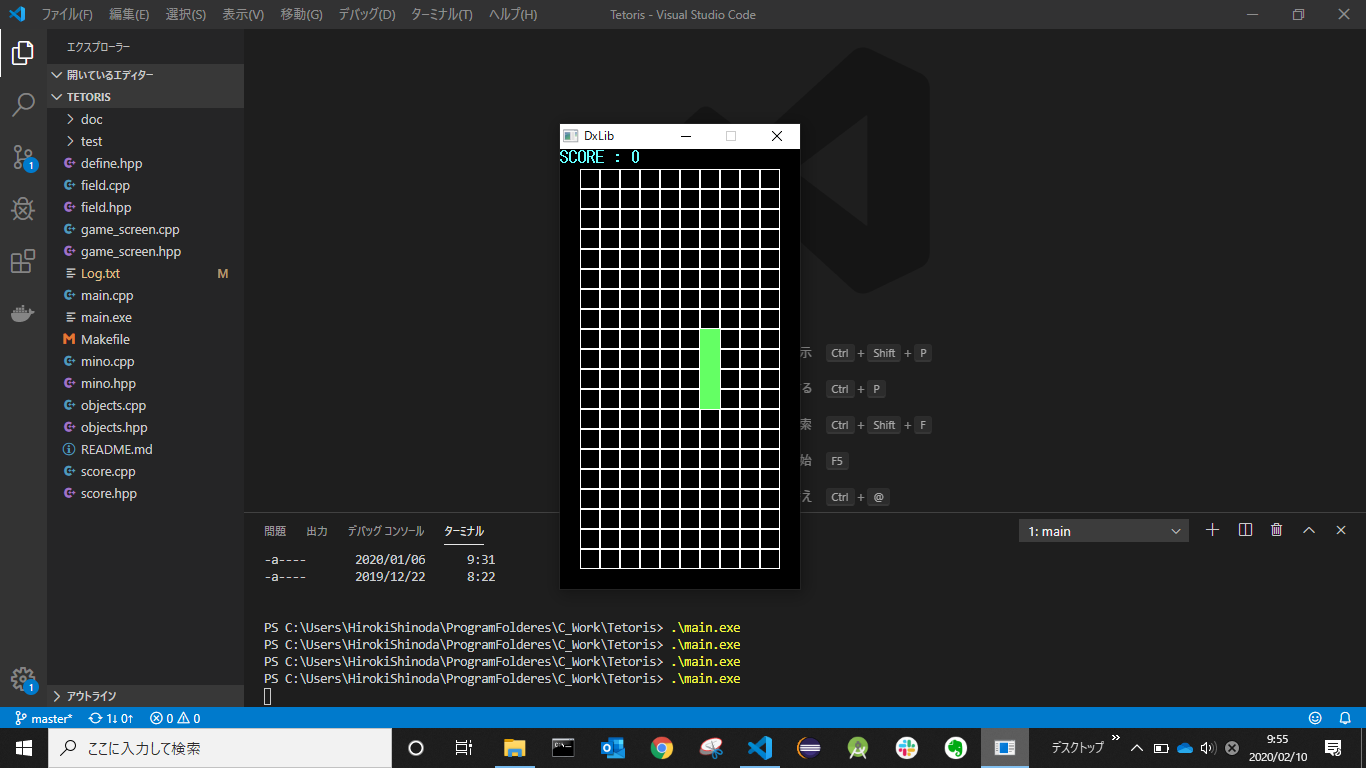
\includegraphics[scale=0.5]{./soft_img/fall.png}
    \caption{テトリミノの落下}
    \label{fool}
  \end{center}
\end{figure}
\begin{figure}[htb]
  \begin{center}
    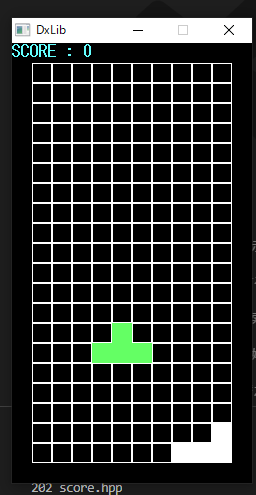
\includegraphics[scale=0.5]{./soft_img/stick.png}
    \caption{テトリミノの固定}
    \label{stick}
  \end{center}
\end{figure}
\begin{figure}[htb]
  \begin{center}
    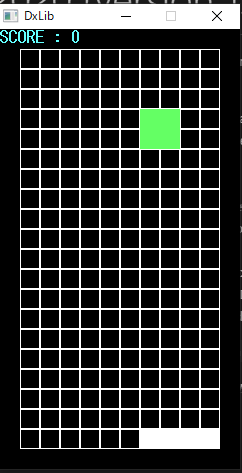
\includegraphics[scale=0.5]{./soft_img/newblock.png}
    \caption{テトリミノの新規作成}
    \label{new}
  \end{center}
\end{figure}
\begin{figure}[htb]
  \begin{center}
    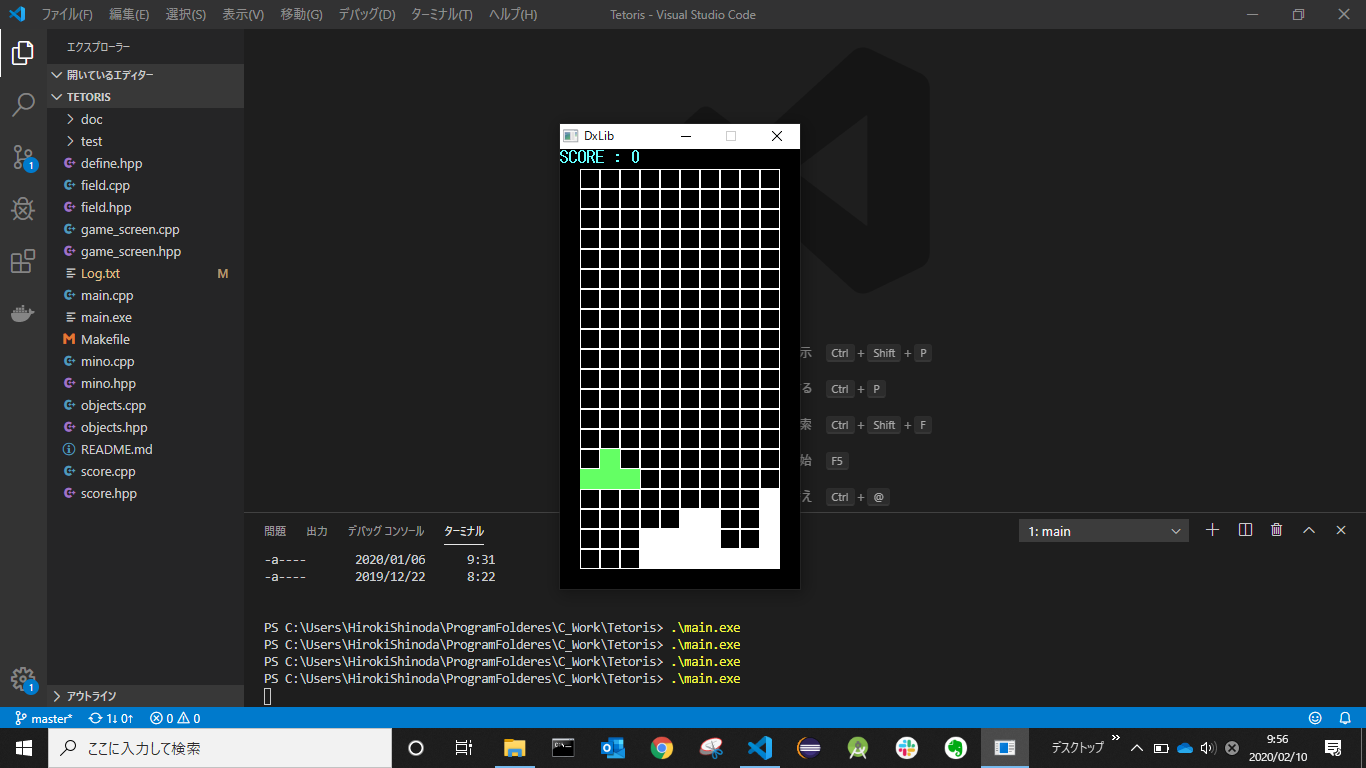
\includegraphics[scale=0.5]{./soft_img/onelinebefore.png}
    \caption{1行消去前の画面}
    \label{one1}
  \end{center}
\end{figure}
\begin{figure}[htb]
  \begin{center}
    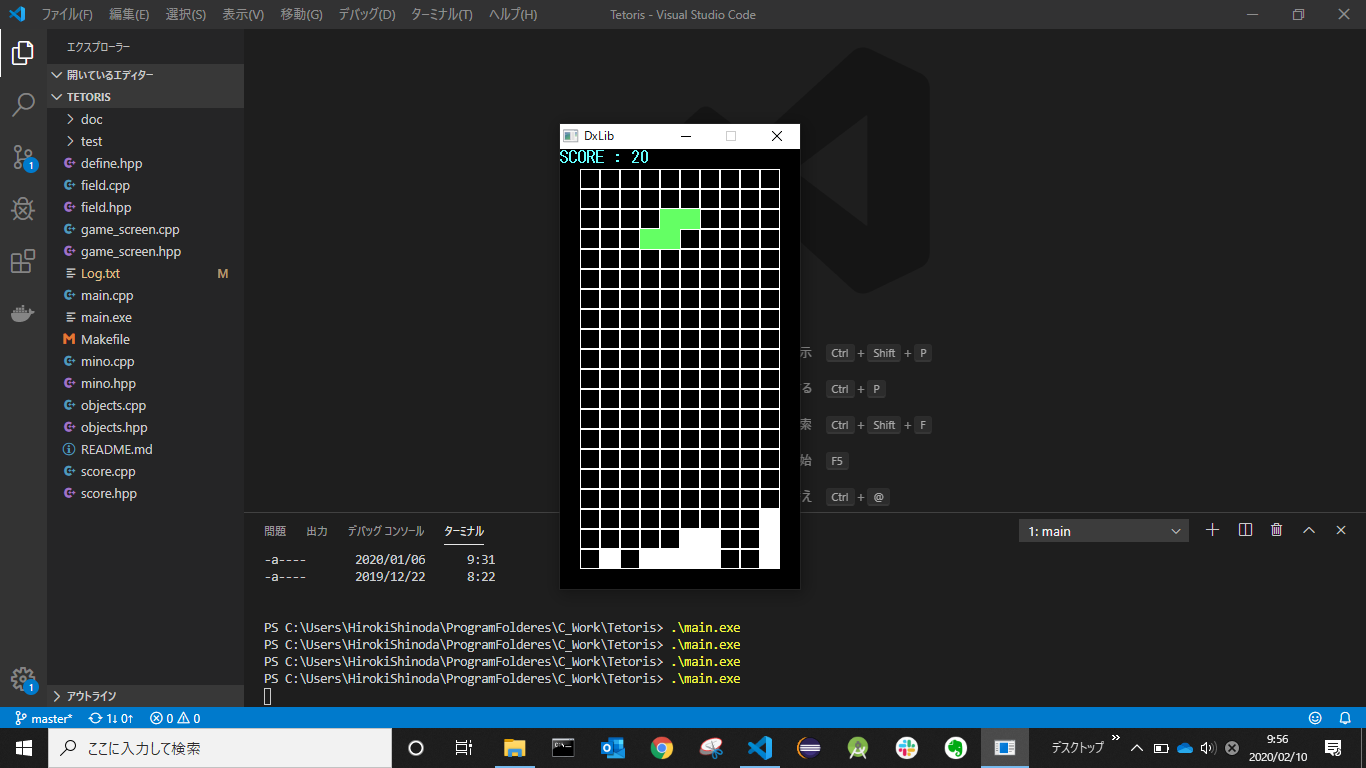
\includegraphics[scale=0.5]{./soft_img/onelineafter.png}
    \caption{1行消去後の画面}
    \label{one2}
  \end{center}
\end{figure}
\begin{figure}[htb]
  \begin{center}
    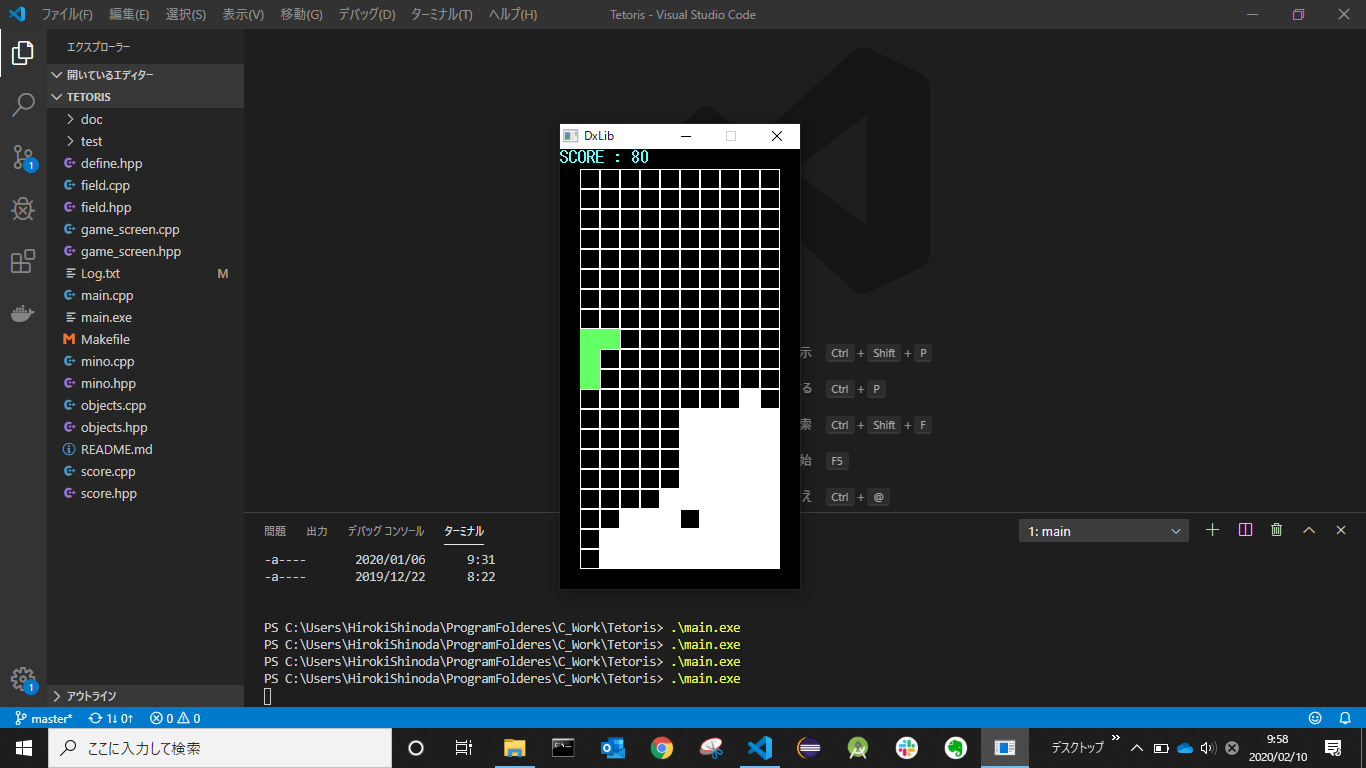
\includegraphics[scale=0.5]{./soft_img/twolinebefore.png}
    \caption{2行消去前の画面}
    \label{two1}
  \end{center}
\end{figure}
\begin{figure}[htb]
  \begin{center}
    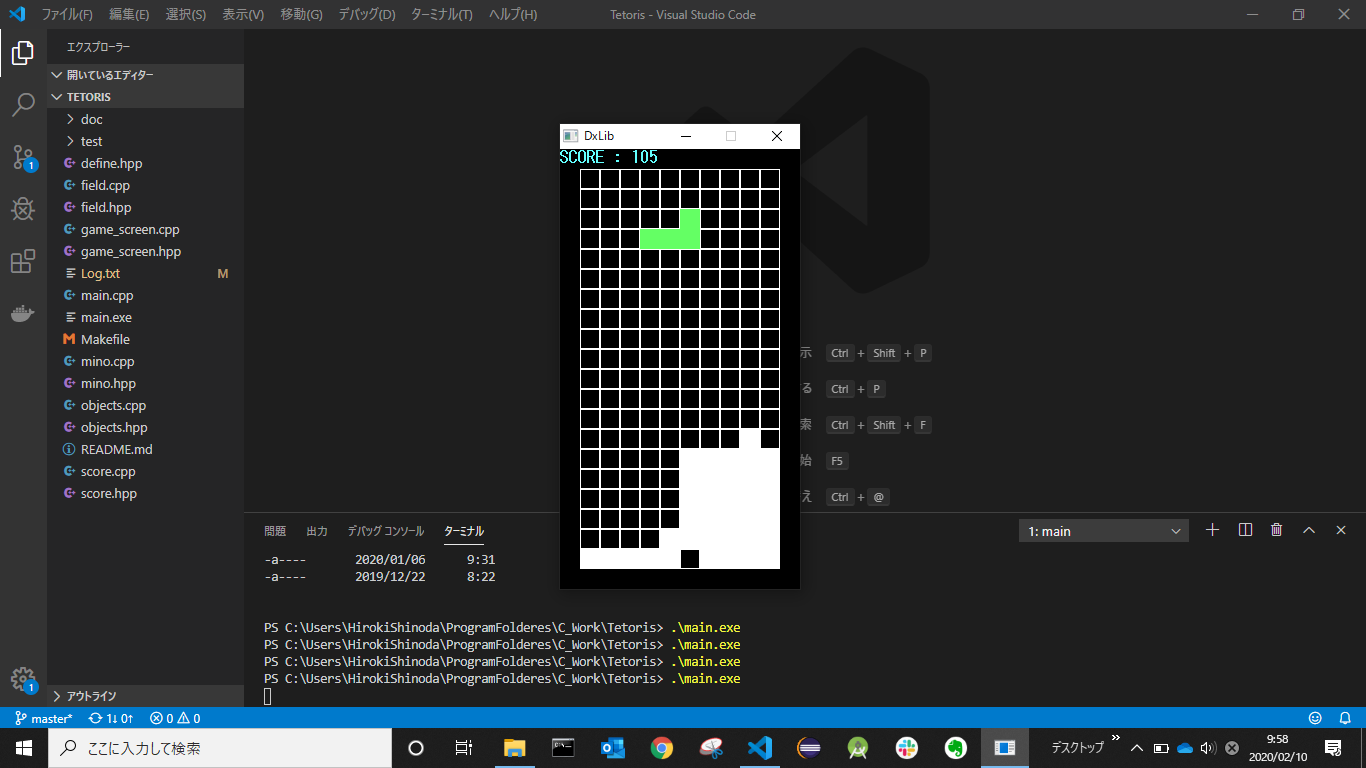
\includegraphics[scale=0.5]{./soft_img/twolineafter.png}
    \caption{2行消去後の画面}
    \label{two2}
  \end{center}
\end{figure}
\begin{figure}[htb]
  \begin{center}
    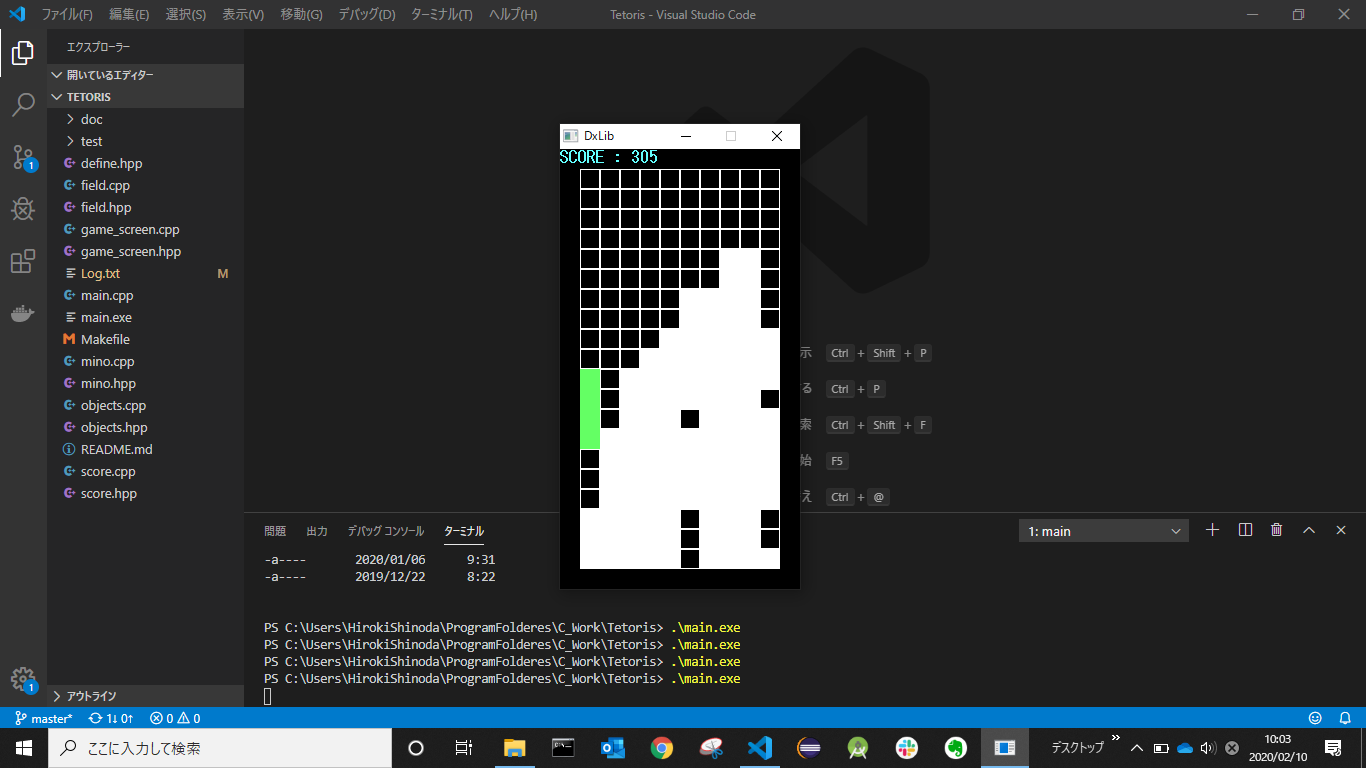
\includegraphics[scale=0.5]{./soft_img/threelinebefore.png}
    \caption{3行消去前の画面}
    \label{three1}
  \end{center}
\end{figure}
\begin{figure}[htb]
  \begin{center}
    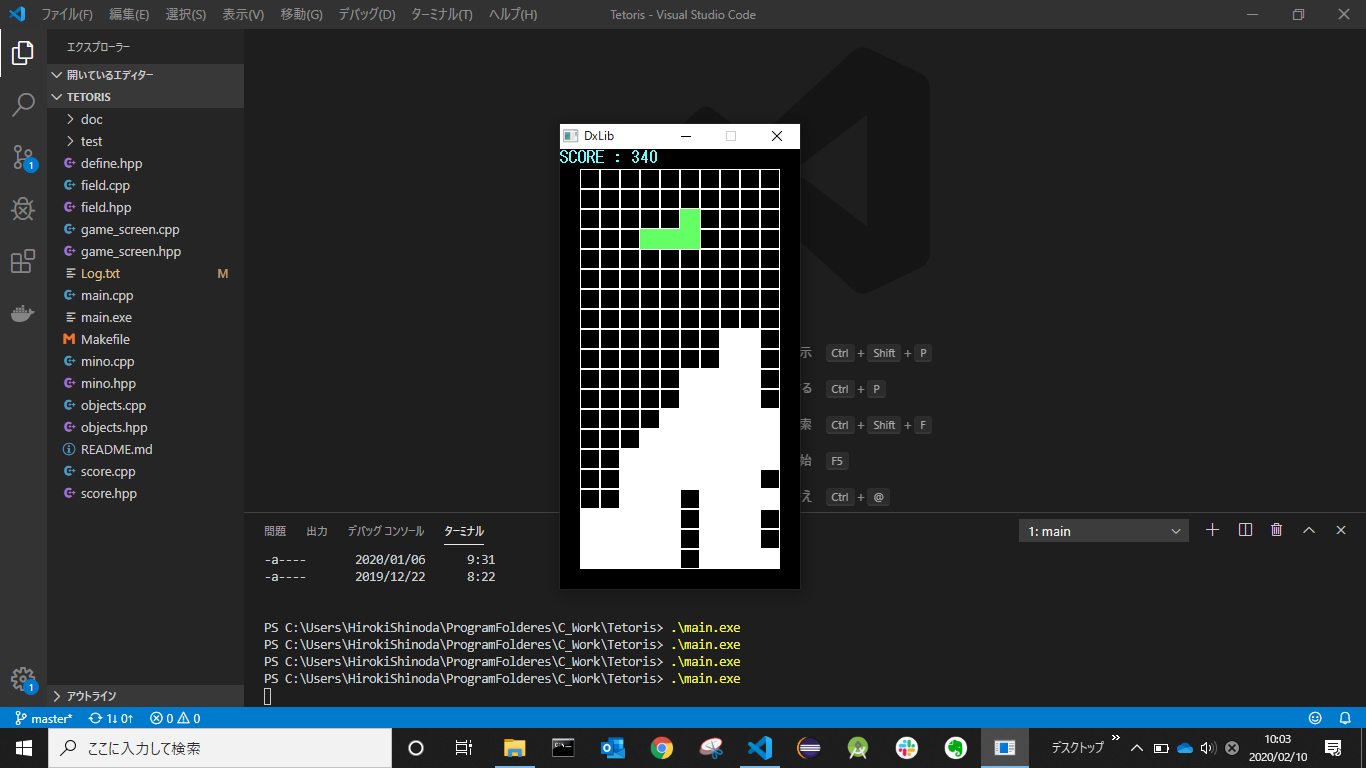
\includegraphics[scale=0.5]{./soft_img/threelineafter.png}
    \caption{3行消去後の画面}
    \label{three2}
  \end{center}
\end{figure}
\begin{figure}[htb]
  \begin{center}
    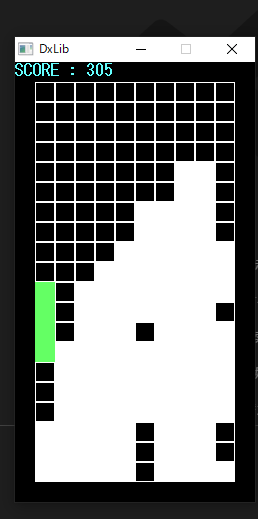
\includegraphics[scale=0.5]{./soft_img/tetorisbefore.png}
    \caption{4行消去前の画面}
    \label{tetoris}
  \end{center}
\end{figure}
\begin{figure}[htb]
  \begin{center}
    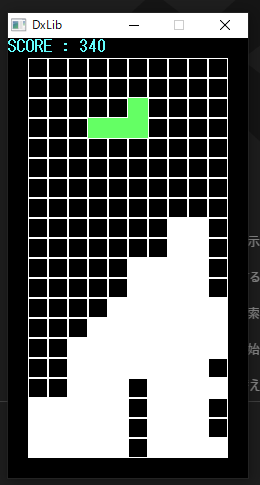
\includegraphics[scale=0.5]{./soft_img/tetorisafter.png}
    \caption{4行消去後の画面}
    \label{tetoris2}
  \end{center}
\end{figure}
\begin{figure}[htb]
  \begin{center}
    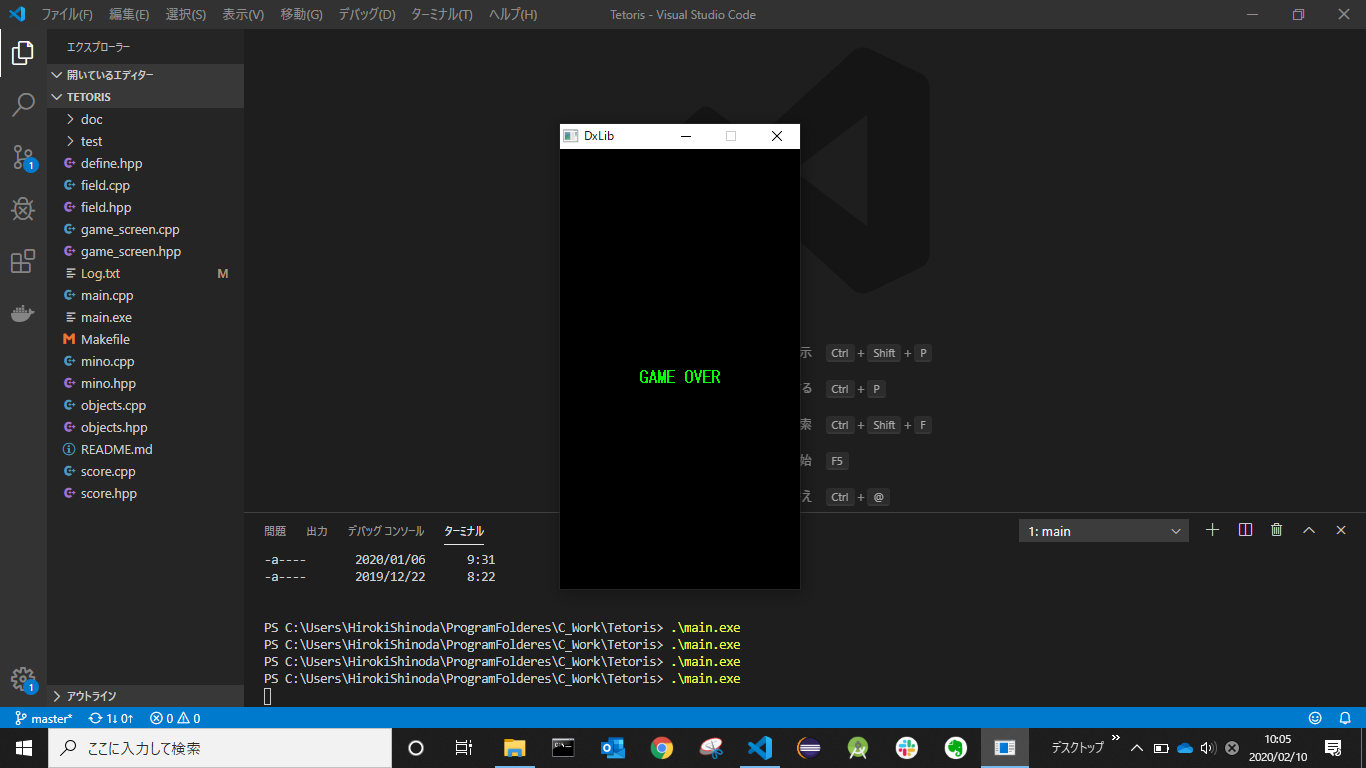
\includegraphics[scale=0.5]{./soft_img/gameover.png}
    \caption{ゲームオーバー画面}
    \label{gameover}
  \end{center}
\end{figure}

  \clearpage
  \section{作成後の批評・考察}
    \subsection{プレイした人の感想}
\begin{itemize}
  \item ブロックが1色じゃないほうが楽しい.
  \item 次に落ちてくるブロックが分かるほうが使いやすい.
  \item ホールド機能が欲しい.
  \item スコアによってスピードが変化するほうが良い.
\end{itemize}

\subsection{改善点}
\begin{itemize}
  \item ブロックを多色にする.
  \item 次に落ちてくるブロックの表示を行う.
  \item ホールド機能を実装する.
  \item 速度の変化を実装する.
\end{itemize}

\subsection{設計・作成に関する反省}
今回は,ウォーターフォール設計を用いてソフトウェアを作成した.
1つ1つの工程で成果が文章化出来た点では,資料作成や日程の管理がやりやすかった.
しかし,バグを発見した際に仕様まで戻る必要があったため予想以上の時間がかかった.
また,最終形にならないとシステムの形が見えてこないので仕様の変更(ユーザーの要求)
には対応しづらいと思った.

  \clearpage
  \section{プログラムリスト}
    %\begin{multicols}{2}
    \lstinputlisting[caption=define.hpp,label=define]
    {../define.hpp}
    \lstinputlisting[caption=field.cpp,label=field]
    {../field.cpp}
    \lstinputlisting[caption=field.hpp,label=field_h]
    {../field.hpp}
    \lstinputlisting[caption=game\_screen.cpp,label=game_screen]
    {../game_screen.cpp}
    \lstinputlisting[caption=game\_screen.hpp,label=game_screen_h]
    {../game_screen.hpp}
    \lstinputlisting[caption=main.cpp,label=main]
    {../main.cpp}
    \lstinputlisting[caption=mino.cpp,label=mino]
    {../mino.cpp}
    \lstinputlisting[caption=mino.hpp,label=mino_h]
    {../mino.hpp}
    \lstinputlisting[caption=objects.cpp,label=objects]
    {../objects.cpp}
    \lstinputlisting[caption=objects.hpp,label=objects_h]
    {../objects.hpp}
    \lstinputlisting[caption=score.cpp,label=score]
    {../score.cpp}
    \lstinputlisting[caption=score.hpp,label=score_h]
    {../score.hpp}
    %\end{multicols}
\end{document}
